% INTRODUCTION
The ocean absorbs $40 \%$ of the anthropogenically produced carbon dioxide (CO$_2$) from the atmosphere \cite{omand_sinking_2020}. 
% Some amount of CO$_2$ is exported to the deep ocean: 
 % In the ocean, most of the transport of carbon from the surface to the deep sea occurs via settling aggregates.
 Phytoplankton, the main organic component of marine aggregates, takes in CO$_2$ during photosynthesis near the surface ocean
%  , and organic or inorganic carbon is dissolved in them. 
Once the phytoplankton and other organic or inorganic matters form an aggregate, it carries the dissolved carbon to the deep ocean. This process removes CO$_2$ from the atmospheric carbon cycle \cite{burd_particle_2009} and plays a role in regulating atmospheric CO$_2$ and climate changes which is one of the most significant environmental problems we face today. 
 Thus, it is critical to understand the dynamics of settling marine aggregates in the oceanic fluid.
 \par
{\color{blue} LITERATURE REVIEW}
 \par
Our research is centered on computing the velocity field of the settling marine aggregates model in an ambient fluid under gravity using boundary integral equation (BIE) formulations. We construct marine aggregates using cubes to capture their fractal shape. A detailed explanation of the modeling is in this chapter, section XX. We consider both homogeneous fluid in chapter 2 and density stratified fluid in chapter 3. 
\par
In chapter 2, we introduce the governing equations and the velocity solutions to the system. This includes the comparison of two BIE formulations. We then show the numerical methods for solving the velocity field and compuations of forces. We analyze the drag, torque, straining forces acting on the different sizes of aggregates with three types of background flows.
 To simulate concentration dynamics, we couple the velocity obtained using the BIE method with the advection-diffusion equation.
\par
In chapter 3, we consider a varying density fluid in the vertical direction. Due to the fluid density gradient, we modify the fluid momentum equation. We also derive the particular velocity solution in addition to the homogeneous solution. Since the new velovity solution has the volume integral term which is computationally expensive to evaluate, we use the fast multipole method (FMM). In section XX, we give a brief introduction to the FMM and its open-source library. 
% The package we use provides the computation related to Laplace and Helmholtz kernel only. We thus modify Laplace kernel to compute our volume integral with the Stokeslet in section 11. The validation of the package and proof of efficiency are also included in this section. 
% We conclude this report with our future research plans in part $\RN{3}$.
\par
{\color{blue} ADD DESCRIPTION OF CHAPTER 4 AND 5}
%
%
%
%===SECTION 1.1=========================================
\section{Aggregate model}
We consider marine aggregates composed of cubic particles, as shown in Figure \ref{fig_cube10}. The dimensionless length of each cube side is $L=2$.
\begin{figure}[ht]
	\begin{center}
		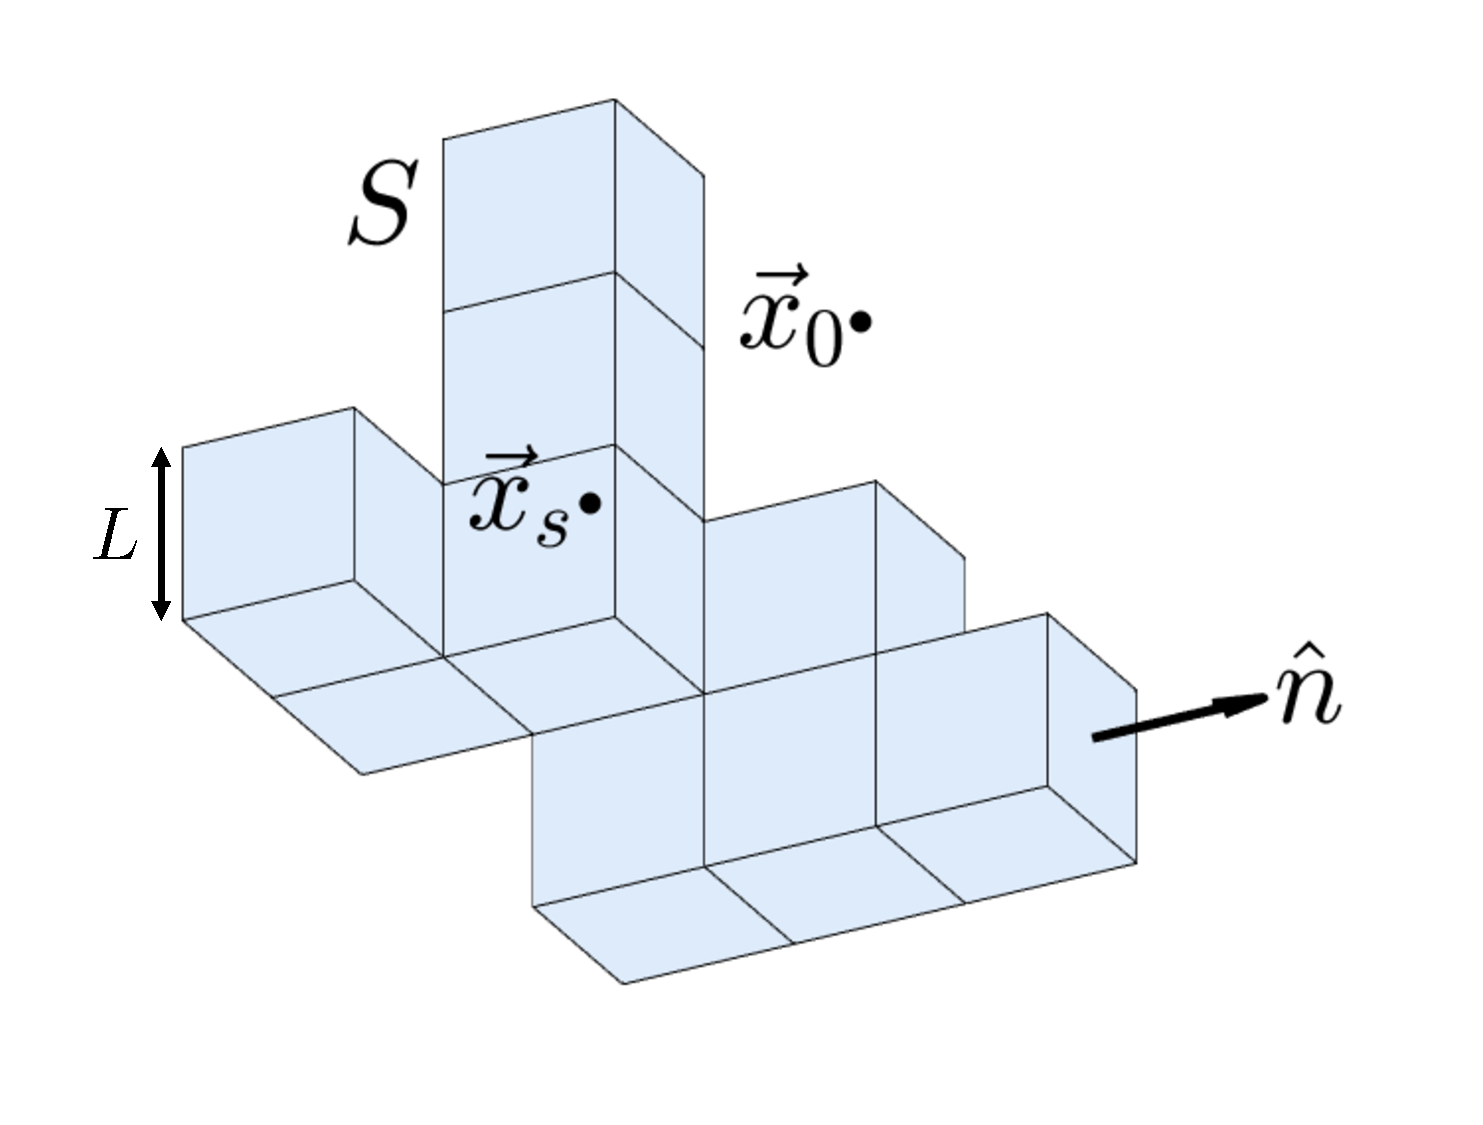
\includegraphics[scale=0.25]{figures/fig_cube10_CC.pdf}
	\end{center}
	\caption{Example aggregate model with 10 cubes. We denote $S$ as the particle surface and $\hat{n}$ as its normal. The vectors $\vec{x}_s$ and $\vec{x}_0$ represent points on and outside of $S$. }
	\label{fig_cube10}
\end{figure}
Since the aggregates have a fractal structure, it is not straightforward to measure their sizes. Two options we consider are the gyration and maximum radii denoted by $R_g$ and $R_m$, respectively. They are defined as,
\begin{equation}
R_g  = \sqrt{\frac{1}{NC} \sum_{i=1}^{NC} \| \vec{x}_i - \vec{x}_{cm} \|^2},
\label{eq_Rg}
\end{equation}
and
\begin{equation}
R_m = 1+ \max_{i = 1, \cdots, NC} \| \vec{x}_i - \vec{x}_{cm} \|,
\label{eq_Rm}
\end{equation}
where $NC$ is the number of cubes in the aggregate, $\vec{x}_i$ is the center of each cube.
We obtain the center of the aggregate, $\vec{x}_{cm}$, by taking mean values of each element of $\vec{x}_i$ for $i = 1, \cdots, NC$.
\par
We obtain randomly shaped aggregates with two different methods that are well established, individually-added-aggregates (IAA) and cluster-to-cluster aggregates (CCA). 
To form an aggregate with IAA method, we introduce a single cube in the periodic box and add another cube, one at a time. For CCA method, on the other hand, we initially position all $N$ cubes, non-adjacent, within the periodic domain and let all cubes undergo an unbiased random walk. If any two cubes form a cluster, the cluster can form another cluster.
Typically, the IAA method gives a more compact form of aggregates, with dimension $\sim 2.56$, than the CCA case which has dimension $\sim 1.79$ \cite{witten_diffusion-limited_1981, kaye_random_2008}.
 We will compare a length scale to the forces acting on the aggregates formed with these two different methods.
%
%
%
%===SECTION 1.2=========================================
\section{Frame of reference}
$\ \ \ \ \ $ 
Throughout this work, we use two frames of reference: 1) lab and 2) moving frame of reference. First, for the fluid velocity computation, we use the lab frame of reference to take advantage of the zero velocity boundary condition at infinity, as shown in Figure \ref{fig_frame_ref} (left). 
\begin{figure}[h]
	\begin{center}
		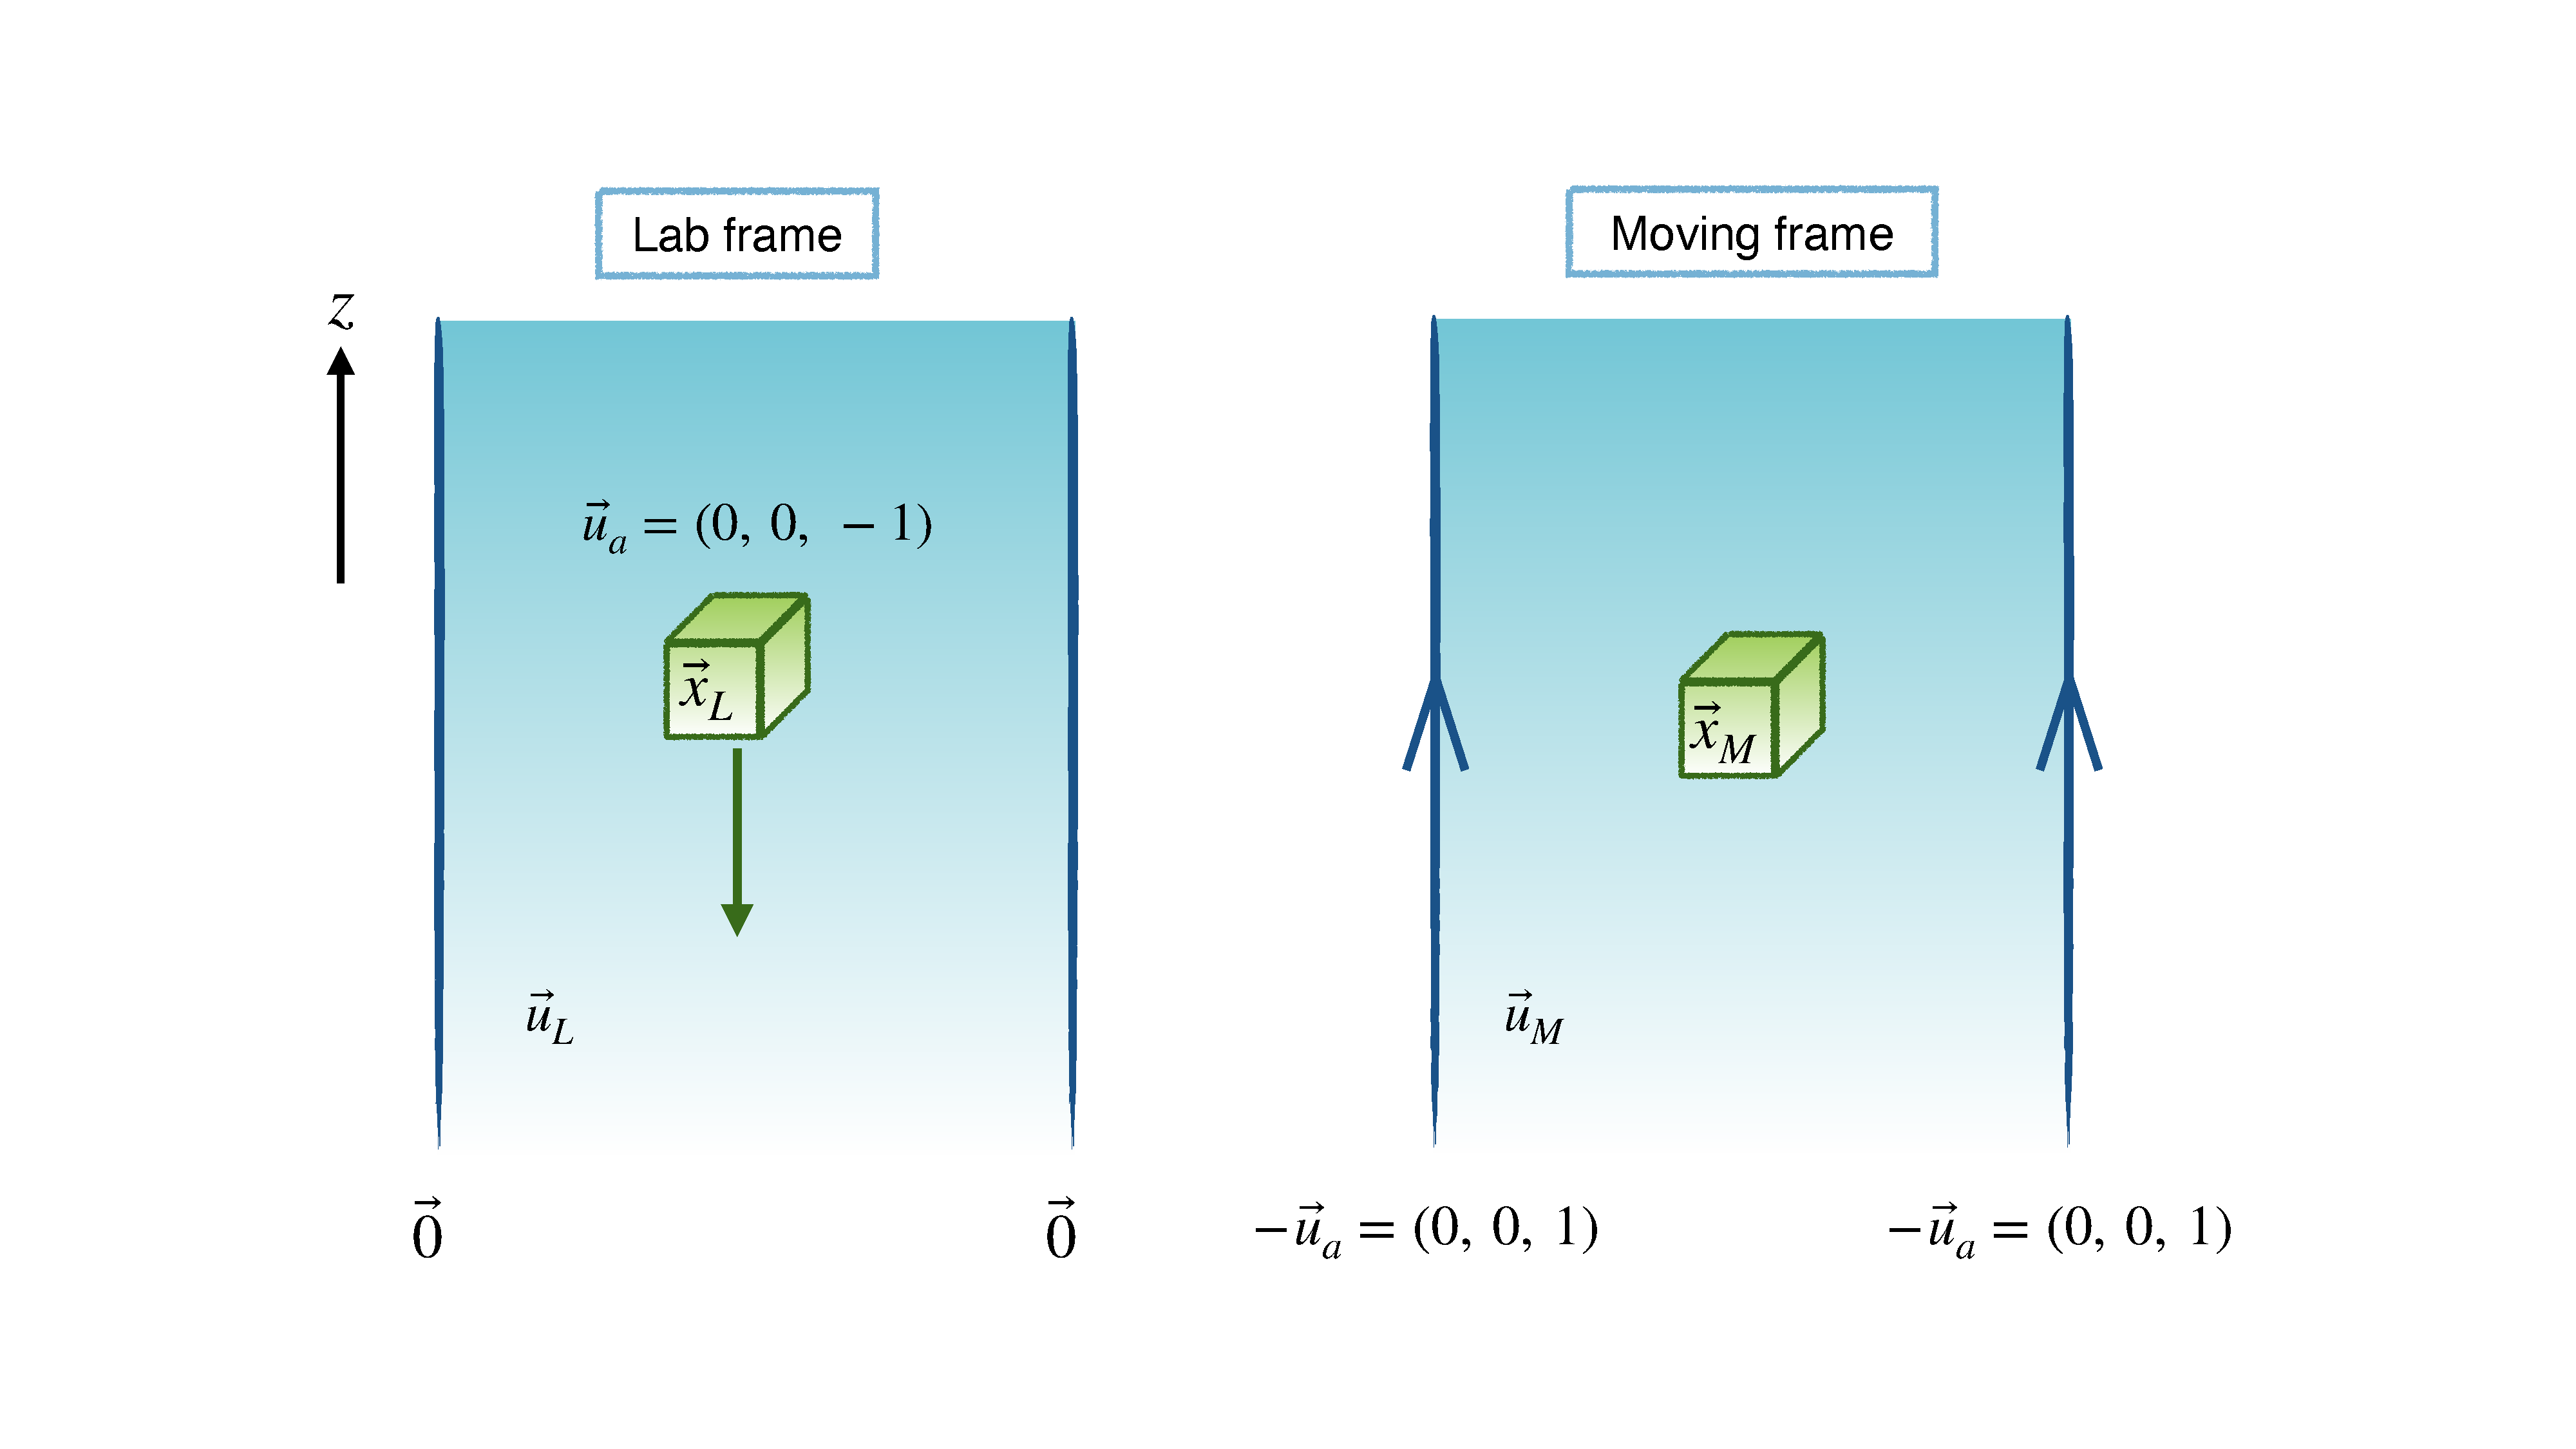
\includegraphics[scale=0.25]{figures/fig_frame_ref}
	\end{center}
	\caption{Schematics of frames of reference. (Left) lab frame and (right) moving frame of reference }
	\label{fig_frame_ref}
\end{figure}
{\color{blue} CHANGE THE FIGURE -> NO FIXED Us}
\\
This condition implies that the domain is large enough, compared to the aggregate.
We solve for the stress on the aggregate boundary, by prescribing the constant velocity or the body force of the aggregate, in order to compute the fluid velocity field. 
% We then solve for the fluid equations.
% Note that the position of the aggregate at time $t$, $\vec{x}_L(t)$, can be expressed as
% \begin{equation}
% \vec{x}_L(t) = \vec{x}_L(0) + \vec{u}_s t.
% \label{eq_xl_pos}
% \end{equation}
% Note that $\vec{u}(\vec{x}, \ t)$ represents the velocity inside of the fluid domain at time $t$.
\par
On the other hand, we use the moving frame to model a concentration dynamics.
In this setting, we fix the aggregate in the middle of the fluid domain and move the fluid upward to describe the settling motion, as shown in Figure \ref{fig_frame_ref} (right).
This can be done by change of variable from the velocities in the lab frame; we simply add $-\vec{u}_s$ to all velocities in the lab frame of reference,
\[
\vec{u}_M = \vec{u}_L - \vec{u}_s.
\]
 The velocity at the boundary of the fluid domain becomes the same speed as $\vec{u}_s$ but in the opposite direction, i.e., $-\vec{u}_s = (0, \ 0, \ 1)$. We also can see that now the aggregate has zero velocity in the moving frame of reference.

 